\begin{frame}
  \frametitle{Euclidean norm \& inner product}
  %% \framesubtitle{}

  \begin{itemize}
  \item The Euclidean norm $\norm[2]{\vu} = \sqrt{\sprod{\vu}{\vu}}$ is
    special because it can be derived from the \h{inner product}:
    \[
    \sprod{\vu}{\vv} \coloneq \vx^T \vy = x_1 y_1 + \dots + x_n y_n
    \]
    where $\vu\equiv_E \vx$ and $\vv\equiv_E \vy$ are the standard coordinates
    of $\vu$ and $\vv$ (certain other coordinate systems also work)%
    \pause\gap
  \item The inner product is a \h{positive definite} and \h{symmetric}
    \h{bilinear form} with the following properties:
    \begin{itemize}
    \item $\sprod{\lambda \vu}{\vv} = \sprod{\vu}{\lambda \vv} = \lambda \sprod{\vu}{\vv}$
    \item $\sprod{\vu + \vu'}{\vv} = \sprod{\vu}{\vv} + \sprod{\vu'}{\vv}$
    \item $\sprod{\vu}{\vv + \vv'} = \sprod{\vu}{\vv} + \sprod{\vu}{\vv'}$
    \item $\sprod{\vu}{\vv} = \sprod{\vv}{\vu}$ (\h{symmetric})
    \item $\sprod{\vu}{\vu} = \norm{\vu}^2 > 0$ for $\vu \neq \vnull$ (\h{positive definite})
    \item also called \h{dot product} or \h{scalar product}
    \end{itemize}
  \end{itemize}
  \addnote{From now on, we will only consider Euclidean norms and metrics,
    omitting the subscript for brevity: $\norm{\cdot} = \norm[2]{\cdot}$.}%
\end{frame}

\begin{frame}
  \frametitle{Angles and orthogonality}
  %% \framesubtitle{}

  \begin{itemize}
  \item The Euclidean inner product has an important \h{geometric}
      interpretation \so angles and orthogonality%
    \pause
  \item \h{Cauchy-Schwarz inequality}:
    \[ \bigabs{\sprod{\vu}{\vv}} \leq \norm{\vu}\cdot \norm{\vv} \]
    \pause\ungap[1.5]
  \item \h{Angle} $\phi$ between vectors $\vu,\vv\in \setR^n$:
    \[ 
    \cos \phi \coloneq 
    \frac{\sprod{\vu}{\vv}}{\norm{\vu}\cdot \norm{\vv}}
    \]
    \ungap
    \begin{itemize}
    \item $\cos \phi$ is the ``cosine similarity'' measure
    \end{itemize}
    \pause
  \item $\vu$ and $\vv$ are \h{orthogonal} iff $\sprod{\vu}{\vv} = 0$
    \begin{itemize}
    \item the \h{shortest connection} between a point $\vu$ and a subspace $U$ is
      orthogonal to all vectors $\vv\in U$
    \end{itemize}
  \end{itemize}
\end{frame}

\begin{frame}[fragile]
  \frametitle{Cosine similarity in R}
  %% \framesubtitle{}

The \texttt{dist()} function does not calculate the cosine measure (because it
is a similarity rather than distance value), but:

\begin{small}
\[
\mathbf{M}\cdot \mathbf{M}^T = 
\begin{bmatrix}
  \cdots & \vu[1] & \cdots \\
  \cdots & \vu[2] & \cdots \\
  \\
  \\
  \cdots & \vu[n] & \cdots 
\end{bmatrix}
\cdot
\begin{bmatrix}
  \vdots & \vdots & & \vdots \\
  \vu[1] & \vu[2] & & \vu[n] \\
  \vdots & \vdots & & \vdots 
\end{bmatrix}
\]
\end{small}
\gap[.5]
\[
\text{\So}\quad
\bigl( \mathbf{M}\cdot \mathbf{M}^T \bigr)_{ij}
= \sprod{\vu[i]}{\vu[j]}
\]

\gap[0]
\begin{alltt}\small
\REM{Matrix of cosine similarities between rows of \textbf{M}:}
> M.norm <- normalise(M, p=2)  \REM{only works with Euclidean norm!}
> M.norm \%*\% t(M.norm)
\end{alltt}
\end{frame}

\begin{frame}[fragile]
  \frametitle{Euclidean distance or cosine similarity?}

  \begin{itemize}
  \item Which is better, Euclidean distance or cosine similarity?
  \item[]
  \item<2-> They are equivalent: if vectors are normalised ($\norm[2]{\vu} = 1$),
    both lead to the same neighbour ranking
  \end{itemize}

  \onslide<3->
  \begin{align*}
    \dist[2]{\vu}{\vv} 
    &= \sqrt{\norm[2]{\vu - \vv}}
    = \sqrt{\sprod{\vu - \vv}{\vu - \vv}}
    \\
    &= \sqrt{\sprod{\vu}{\vu} + \sprod{\vv}{\vv} - 2 \sprod{\vu}{\vv}}
    \\
    &= \sqrt{\norm[2]{\vu} + \norm[2]{\vv} - 2 \sprod{\vu}{\vv}}
    \\
    &= \sqrt{2 - 2 \cos \phi}
  \end{align*}
\end{frame}

\begin{frame}[c]
  \frametitle{Euclidean distance and cosine similarity}

  \begin{center}
    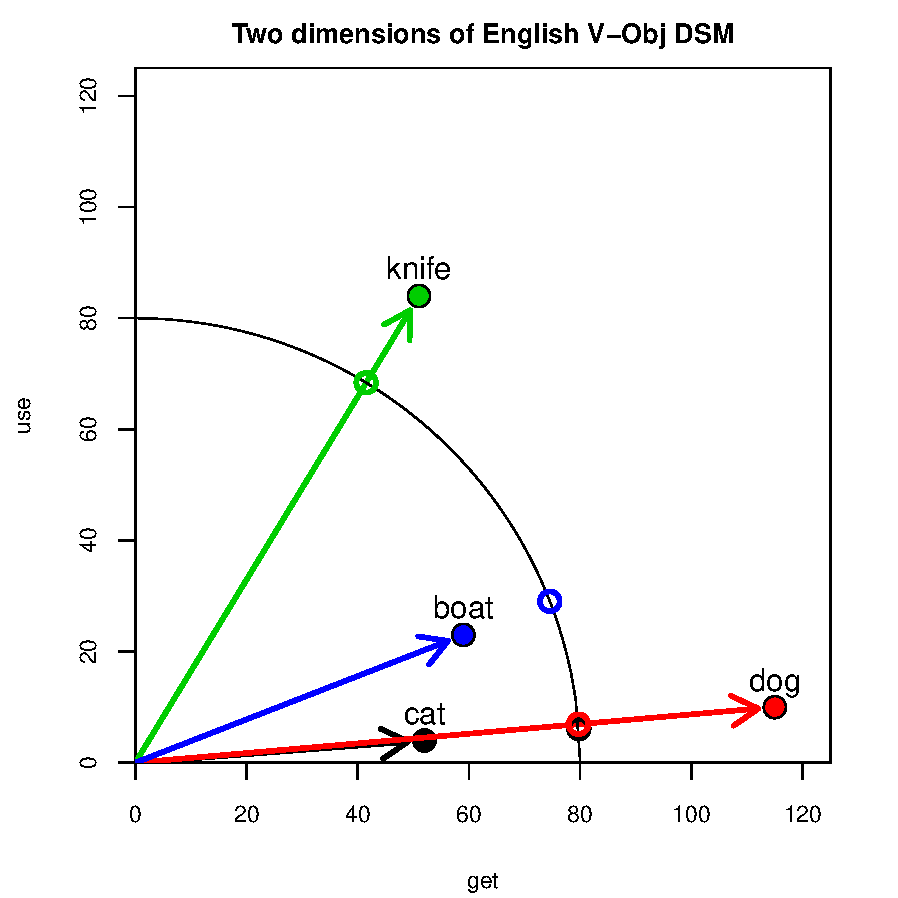
\includegraphics[width=7cm]{img/hieroglyph_2d_4}
  \end{center}
\end{frame}


\begin{frame}
  \frametitle{Cartesian coordinates}
  %% \framesubtitle{}

  \begin{itemize}
  \item A set of vectors $\vb[1], \ldots, \vb[n]$ is called \h{orthonormal} if
    the vectors are pairwise orthogonal and of unit length:
    \begin{itemize}
    \item $\bigsprod{\vb[j]}{\vb[k]} = 0$ for $j\neq k$
    \item $\bigsprod{\vb[k]}{\vb[k]} = \bignorm{\vb[k]}^2 = 1$
    \end{itemize}
  \item An orthonormal basis and the corresponding coordinates are called
    \h{Cartesian}%
    \pause
  \item Cartesian coordinates are particularly intuitive, and the inner
    product has the same form wrt.\ every Cartesian basis $B$: for $\vu\equiv_B
    \vx'$ and $\vv\equiv_B \vy'$, we have
    \[ \sprod{\vu}{\vv} = (\vx')^T \vy' = x'_1 y'_1 + \dots + x'_n y'_n \]
  \item NB: the column vectors of the matrix $\mathbf{B}$ are orthonormal%
    \begin{itemize}
    \item recall that the columns of $\mathbf{B}$ specify the standard
      coordinates of the vectors $\vb[1], \ldots, \vb[n]$
    \end{itemize}
  \end{itemize}
\end{frame}

\begin{frame}
  \frametitle{Orthogonal projection} 
  %% \framesubtitle{}
  
  \begin{itemize}
  \item Cartesian coordinates $\vu \equiv_B \vx$ can easily be computed:
    \begin{align*}
      \sprod{\vu}{\vb[k]} &= \sprod{\sum_{j=1}^n x_j \vb[j]}{\vb[k]} \\
      &= \sum_{j=1}^n x_j \underbrace{\sprod{\vb[j]}{\vb[k]}}_{= \delta_{jk}} 
      = x_k
    \end{align*}
    \begin{itemize}\ungap
    \item Kronecker delta: $\delta_{jk} = 1$ for $j=k$ and $0$ for $j\neq k$
    \end{itemize}
    \pause\gap
  \item \h{Orthogonal projection} $P_V:\setR^n\to V$ to subspace $V
    \coloneq \Span{\vb[1], \ldots, \vb[k]}$ (for $k < n$) is given by
    \[
    P_V \vu \coloneq \sum_{j=1}^k \vb[j] \sprod{\vu}{\vb[j]}
    \]
  \end{itemize}
\end{frame}

%%% Local Variables: 
%%% mode: latex
%%% TeX-master: "../../workspace"
%%% End: 
